\documentclass{kththesis}

\usepackage{blindtext} % This is just to get some nonsense text in this template, can be safely removed

\usepackage{csquotes} % Recommended by biblatex
\usepackage{biblatex}
\addbibresource{references.bib} % The file containing our references, in BibTeX format

%added by me:
\usepackage{xcolor}
\usepackage{color}
\usepackage{amsmath,float}
\usepackage{caption}
\captionsetup[figure]{labelfont=bf}
\usepackage{amsthm}
\theoremstyle{definition}
\newtheorem{definition}{Definition}[section]
\newtheorem{hyp}{Hypothesis}
\newtheorem{RQ}{Research Question}[section]

\usepackage{graphicx}


%for clickable hyperlinks
%colors for different links
\usepackage{hyperref}
\hypersetup{
    colorlinks,
    linkcolor={red!50!black},
    citecolor={blue!50!black},
    urlcolor={blue!80!black}
}

\usepackage{cleveref}

\graphicspath{{Imgs/}}

\title{Competitive self-playing reinforcement learning agents used in the Nordic stock market, to understand market microstructure}

\alttitle{Reinforcement learning agenter i den nordiska aktiemarknaden, för att förstå marknadens mikrostruktur }
\author{Marcus Elwin}
\email{elwi@kth.se}
\supervisor{Hamid Reza Faragardi}
\examiner{Elena Troubitsyna}
\programme{Master of Science in Machine Learning}
\school{School of Electrical Engineering and Computer Science}
\date{\today}



\begin{document}


% Frontmatter includes the titlepage, abstracts and table-of-contents
\frontmatter

\titlepage

\begin{abstract}
  English abstract goes here.

\end{abstract}


\begin{otherlanguage}{swedish}
  \begin{abstract}
    Svensk sammanfattning
  \end{abstract}
\end{otherlanguage}


\tableofcontents


% Mainmatter is where the actual contents of the thesis goes
\mainmatter


\chapter{Introduction}

%We use the \emph{biblatex} package to handle our references.  We therefore use the
%command \texttt{parencite} to get a reference in parenthesis, like this
%\parencite{heisenberg2015}.  It is also possible to include the author
%as part of the sentence using \texttt{textcite}, like talking about
%the work of \textcite{einstein2016}.

\section{Background}
Modern financial markets such as NASDAQ, CME and NYSE have all been effected by the rise and presence of \textit{Algorithmic Trading} and \textit{High-Frequency Trading} (HFT).  Where both types of trading consists in using computer programs to implement investment and trading strategies \parencite{abergel2012market}. These types of strategies have according to \textcite{abergel2012market, o2015high} raised various questions about there effects on the financial markets. Mainly in areas as: \textit{liquidity, volatility, price discovery, systematic risk, manipulation} and \textit{market organization}. Where a quite recent example of the proposed effect of algorithmic trading and HFT on financial markets is \textit{the Flash Crash} in the 6th of May 2010. Where in the course of 30 minutes U.S. stock market indices, stock-index futures, options, and exchange-traded funds. Experienced a sudden price drop of more than five percent,followed by a rapid rebound \parencite{kirilenko2011flash,kirilenko2017flash}. See an illustration of this in \autoref{fig:1}.
\newline
\newline
Trading in the financial market can be seen as a search problem where buyers and sellers search for each-other. Which depends on market structure \parencite{abergel2012market}. \textit{Market microstructure} is a branch of economics, where one tries to understand trading dynamics on the financial market on a micro level \parencite{o1995market, hasbrouck2007empirical}. Market microstructure theory is used by regulators, traders and organizers of financial markets. In order to make a profit or create more transparent and efficient markets. Where a recent regulation with the purpose of making markets more transparent and efficient is \textit{Markets in Financial Instruments Directive} (MiFID) II \parencite{busch2016mifid}.

\begin{figure}[ht]
    \centering
    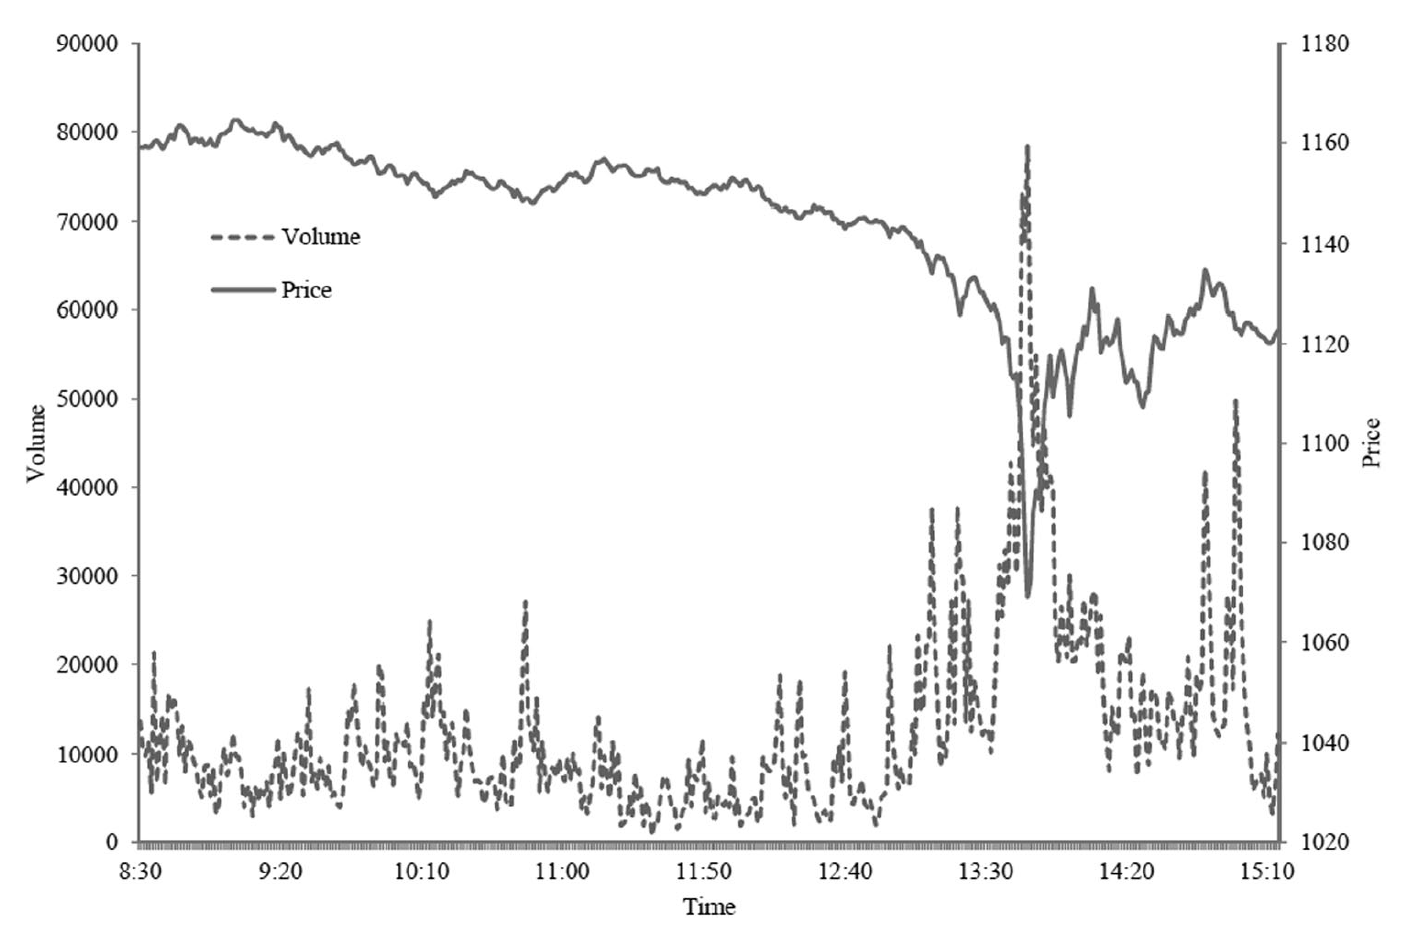
\includegraphics[scale=.7]{flashcrash.PNG}
    \caption{Minute-by-minute transaction prices and trading volume on E-mini S\& P futures contracts during the flash crash, between 8:30 to 15:15. Notice the distinct drop and rebound at the end of the day. Source: \textcite{kirilenko2017flash} }
    \label{fig:1}
\end{figure}

However as mentioned by \textcite{o2015high} due to HFT and algoritmic trading. Learning models and empirical models used in market microstructure in the past are deficient and may not longer be appropriate. Which calls for the use of new more capable methods. Where \textit{Reinforcement Learning} and other machine learning methods are of great interest. Machine learning and AI has been used in a financial setting for some time, and has become ubiquitous in finance today. Mainly due to the abundance of available data and computing power. 
\newline
\newline
Where recent achievements for the use of Reinforcement Learning has been seen in the game Go with \textit{AlphaGo, AlphaGoZero} \parencite{silver2016mastering} programs being able to win over esteemed Go champions. More complicated strategic games as Star Craft has also seen successful application of reinforcement learning \parencite{vinyals2017starcraft}. Therefore the focus of this thesis will be to examine the possibility of using deep reinforcement learning and competitive self-play. In order to understand the market microstructure on a simulated Nordic stock market.

%need to work with
\section{Research Question}
The research question for this thesis is shown below:

\begin{RQ}
Will trading dynamics such as the bid-ask spread clustering, optimal trade execution and optimal inventory costs be exhibited \& learned by reinforcement learning agents using competitive self-play on a simulated Nordic stock market.
\end{RQ}

\section{Problem}
With more granular and high frequency data as well as more sophisticated trading algorithms. The financial markets has become harder to understand during the past decade. Traditional methods used in market microstructure might have become obsolete as mentioned in \textcite{o2015high}. A traditional supervised learning approach is not of use for this thesis. Due to the fact of the financial markets dynamic nature as a complex system. The agents must be able to adapt and dynamically learn optimal behaviour.  Therefore the problem in this thesis is to understand by using reinforcement learning, specially learning via competitive self-play. On a simulated Nordic stock market. 
\newline
\newline
If common market microstructure trading dynamics such as \textit{bid-ask spread clustering, optimal trade execution} and \textit{optimal inventory costs} as described in \textcite{o1995market}. Will be exhibited and understood by the reinforcement learning agents. Also it is of interest to see what happens with the agents when changing the market conditions. Much like what is happening in the real markets. For example changing the number of participants, order sizes, prices and trading rules.

%\section{Aim}

%\newpage

\section{Objective}
The objective for this thesis is two-fold. Firstly in the case of the principal the objective is to have a functional and working exchange simulator (EXSIM). Where they can change different parameters, policies, reward functions and other things effecting the market. In order to study and simulate modern financial markets on a microscopic level. Secondly from the thesis point of view, the objective is to investigate the following:

\begin{itemize}
    \item Can competitive self-play and reinforcement learning be successfully used in a financial setting. 
    \item Can new insight and applications be provided to the the growing field of market microstructure. 
    \item Can reinforcement learning work in more complicated environments such as the financial market.
\end{itemize}


\section{Delimitation}

\section{The principle}

\section{Disposition}

%The student displays knowledge of theoretical background and previous related work (significant literature is mentioned and relevant material is used).

The background is coherent and relevant.
\chapter{Background}
In this chapter relevant theory is presented in order to give the reader a good overview of the fields study during the pre-study that are relevant for the thesis. We begin with .. and finally end with a section on previous related work.

%Necessary
%\section{Modern Financial Markets}

%Ho stoll model for invetory market

%GM

% Daz model for informed traders

% Real market with matching engine e.g. parity
\section{Market Microstructure}
\textit{Market microstructure} is the study of the process and outcomes of exchanging assets under implicit trading rules as mentioned in \textcite{o1995market}. A lot of market microstructure research according to \textcite{madhavan2000market} are concerned with : 
\begin{enumerate}
    \item \textit{Price formation and discovery} i.e. looking in to the black box of the market by which latent demands are translated into prices.
    \item \textit{Market structure and design} i.e. what different rules effect the black box of the market.
    \item \textit{Information and disclosure} i.e. how the workings of the black box affects the behaviour of traders and strategies.
\end{enumerate}
All of these will be covered in this section.

%\newpage

\subsection{Market Participants}
A \textit{market} is the place where traders gather to trade \parencite{harris2003trading} different types of instruments as common stocks, bonds, futures, options, derivatives and foreign exchange rates just to mention a few.
Looking at today's financial markets
\textcite{cartea2015algorithmic} broadly categories three primary classes of traders (or strategies) that partake in the market:
\begin{itemize}
    \item \textbf{Fundamental traders:} those who are driven by economic fundamentals outside the exchange.
    \item \textbf{Informed traders:} traders who profit from leveraging information not reflected in market prices and trading assets in the hope of their increase or decrease in value.
    \item \textbf{Market Makers:} professional trader who profit from facilitating exchange in a particular asset and exploit their skills in executing trades.
\end{itemize}

\subsection{Trading Mechanisms}
Any trading mechanism can be seen as a type of trading game in which players meet virtually or physical at some venue and act according to some rules \parencite{o1995market}. Where the players are some of the participants mentioned in the previous section. The venue or the market is trades are actually happening which can be on an exchange or via other intermediaries. A common division of market structure is presented in \textcite{foucault2013market} \textit{the limit order market} (auction market) and \textit{the dealer market}. In fact all trading mechanisms can be viewed as a variation of these \parencite{foucault2013market}.
\newline
\newline
In limited order markets, the final investors interact directly; there bids and offers are accumulated in the \textit{limited order book} (LOB). By price priority and secondly time priority \parencite{hasbrouck2007empirical}. Whilst in dealer markets participants can only trade at the bid and ask quotes posted by specialized intermediaries i.e. \textit{dealers} or \textit{market makers} \parencite{foucault2013market}. Note that the LOB is very dynamic as it constitutes of \textit{limit orders}\footnote{A limit order is an order that specifies a direction, quantity and acceptable price.}. Which can be cancelled or modified at any time, thus the LOB can change be changed extremely rapid \parencite{hasbrouck2007empirical}. An example of a limit order book is shown below in \autoref{fig:2}.
\begin{figure}[H]
    \centering
    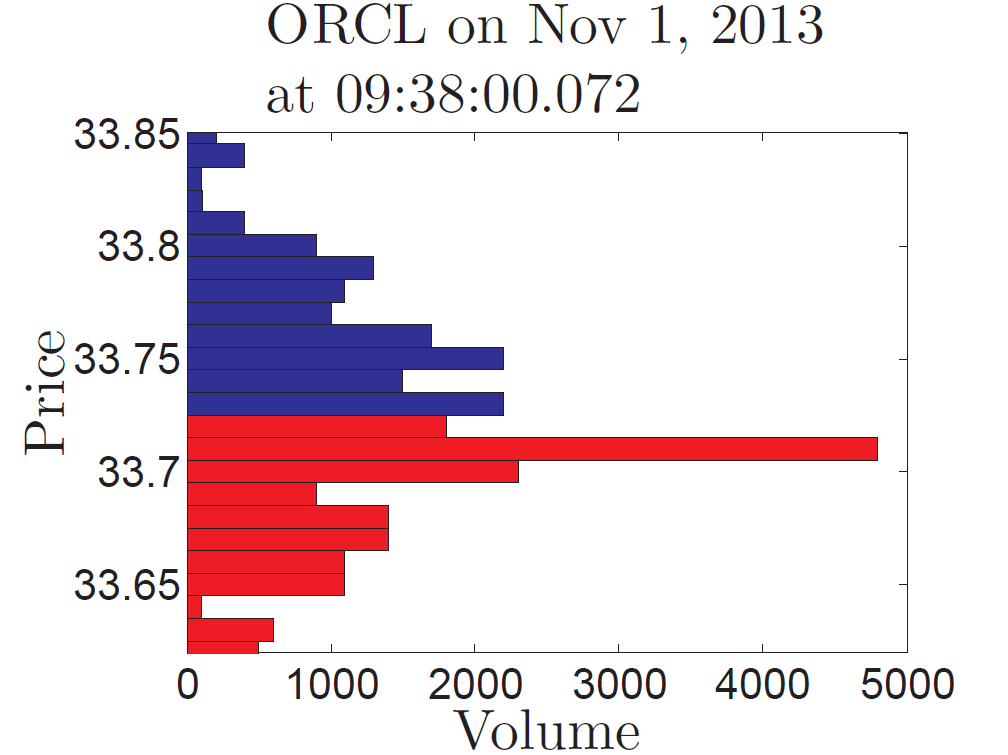
\includegraphics[scale=.65]{LOBex.PNG}
    \caption{Snapshot of the LOB for the ticker ORCL (Oracle) after the 10 000th event during that day. Blue bars indicates sell limit orders, whilst red bars are buy limit orders.}
    \label{fig:2}
\end{figure}
Market orders are other types of orders found on LOB markets, which are usually considered to be more aggressive. This as they seek to execute a trade immediately \parencite{cartea2015algorithmic}. For instance if a market order is placed and the quantity is larger then quantity available in the book. The order is \textit{re-routed} or sad to 'walk the book' until the order is filled \parencite{hasbrouck2007empirical,cartea2015algorithmic}.To make things more complicated modern markets has a lot of different order types. Such as \textit{hidden, reserved, iceburg} and \textit{Fill-or-Kill} orders just to mention a few. Where \parencite{foucault2013market, cartea2015algorithmic, hasbrouck2007empirical} gives a good overview of these. There also exist \textit{hybrid markets} which are traditional quote-driven markets as Nasdaq and London Stock Exchange (LSE) \parencite{foucault2013market}.

\subsection{Price Formation \& Discovery}
The mechanism of price formation is at the very heart of economics.  Which is also important to understand 'stylized facts' in financial price series as \textit{heavy tails} and \textit{volatility clustering}  \parencite{abergel2012market}. \text{Price discovery} is the speed and accuracy with which transactions prices incorporate information available to market participants \parencite{foucault2013market}. In fact market makers, professional traders who stand willing to buy or sell securities. Is a logical starting point for how prices are actually determined in the market \parencite{madhavan2000market}. Another key is also the role of information and who has it, that will be covered more in section .. \parencite{cartea2015algorithmic}.

\begin{figure}[H]
    \centering
    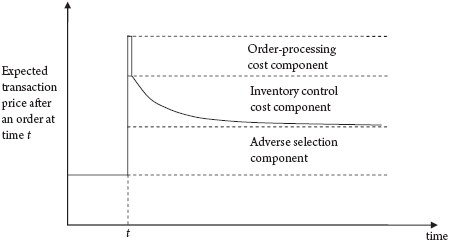
\includegraphics[scale=1]{bidask.png}
    \caption{Three components of bid-ask spread in short-term and lon-term response to a market buy order. Source: \textcite{foucault2013market}}
    \label{fig:3}
\end{figure}

\subsubsection*{Bid-Ask Spread}

The bid-ask spread is usually decomposed into three components: \textit{adverse selection, order-processing costs} and \textit{inventory holding costs} \parencite{foucault2013market}. Order processing costs, consists of the setup price and operating costs of trading. Inventory costs is cost associated with carrying inventory. Adverse selection costs are costs that arise because some traders are more informed then others. When trading with these \textit{informed traders}, market makers will on average lose money \parencite{darley2007nasdaq}. Therefore a fraction of the bid-ask spread can be seen as a compensation for having to trade against informed traders \parencite{darley2007nasdaq}.In \autoref{fig:3} above these are illustrated on a short-term and long-term perspective.
\newline
\newline
Market makers quote two prices the bid price and the ask price where the difference between these is the market makers \textit{spread} \parencite{madhavan2000market}. By doing this market makers are also providing \textit{liquidity} to the market. Spreads measure the execution cost of small transaction, by measuring how close the price of a trade is to the \textit{market price}. Where the market price is the \textit{equilibrium price} i.e. the price where demand equals supply \parencite{cartea2015algorithmic}. One approach is by using the \textit{midprice} in \autoref{eq:1}:

\begin{equation}
    \label{eq:1}
    S_{t} = \frac{1}{2}(a_t + b_t)
\end{equation}
Which is the simple average of the bid ($b_t$) and ask($a_t$) price.
However the most common spread measures are the \textit{quoted} and the \textit{effective} \parencite{cartea2015algorithmic, foucault2013market} spread both shown in \autoref{eq:2} and \autoref{eq:3}

\begin{equation}
    \label{eq:2}
    QS_t = a_t - b_t
\end{equation}

\begin{equation}
    \label{eq:3}
    ES_t = a_t - S_t \text{ or } ES_t = S_t - b_t
\end{equation}
The quoted spread represents the potential cost of immediacy at any point in time as well as the distance from the market price \parencite{cartea2015algorithmic}. As mentioned in \textcite{foucault2013market} the quoted spread is also a good measure of trading costs for small orders used for measuring liquidity. If we normalize \autoref{eq:2} with the mid price we get the \textit{relative quoted spread} 

\begin{equation*}
    RQS_t = \frac{a_t - b_t}{S_t}.
\end{equation*}
Another related measure is the so called \textit{relative weighted average bid-ask spread} (RTWAS):

\begin{equation}
\label{eq:4}
    RTWAS_{t} = \frac{\bar{a}(q) - \bar{b}(q)}{S_t}
\end{equation}
Where $\bar{a}(q)$ and $\bar{b}(q)$ is the average execution price for buy and sell market orders of size $q$ \parencite{foucault2013market}. On the other hand the effective spread or half-spread measures the realized difference between the price paid and the midprice. Which can also be negative indicating that one is buying at a price below or selling above the 'market price' \parencite{cartea2015algorithmic}. ES and QS differ in the fact that ES can only be measured when there is a trade while QS are always observable \parencite{cartea2015algorithmic}.Some stylized facts know about the bid-ask spread are \parencite{hasbrouck2007empirical, madhavan2002market}:
\begin{itemize}
    \item The trade prices series is a martingale
    \item The order flow is not symmetric
    \item The spread declines over time
    \item The bid-ask spread are lower in high volume securities and wider for more riskier securities.
    \item The orders are serially correlated
    \item There is a price impact of trades
\end{itemize}

\subsubsection*{Liquidity}
If the structure of a securities market is compared to a car design, measuring liquidity is like assessing the car's driving performance \parencite{foucault2013market}.Liquidity impounds the usual economic concept of \textit{elasticity}. In a liquid market, a small shift in supply and demand doesn't result in large price changes \parencite{hasbrouck2007empirical}. However liquidity is also concerned with trading costs. Market makers are seen as liquidity providers (sell-side) whilst liquidity demanders are the customers (buy-side) \parencite{hasbrouck2007empirical}. A key dimension of liquidity is \textit{immediacy}. This is the ability of a investor to buy or sell an asset without having to wait to find a counterpart. With an offsetting position to sell or buy \parencite{cartea2015algorithmic}. In fact the bid-ask spread is a common measure of how liquid a market is \parencite{foucault2013market}.

\subsubsection*{Other measures of implicit trading costs}
A popular benchmark in trading costs analysis is the \textit{volume-weighed average price} (VWAP). For all transaction in the stock during a interval ($T$), often a trading day \parencite{foucault2013market}:

\begin{equation}
    \label{eq:5}
    VWAP = \sum_{t\in T}{w_t p_t}
\end{equation}
Where $w_t = \frac{|q_t|}{\sum_{t\in T}{|q_t|}}$ and $p_t$ and $q_t$ is the price and size of the $t^{th}$ trade. Investors evaluate their broker's performance in getting a good price for their order, by comparing their own price with the day's VWAP \parencite{foucault2013market}. Another concern for participants that wish to execute large orders, is that they will have an adverse \textit{price impact}. That is, increasing the price when buying aggressively and lowering it when selling \parencite{cartea2015algorithmic}. A normal way of measuring this, is running a regression on the change of the midprice of the form below:

\begin{equation}
    \label{eq:6}
    \Delta S_n = \lambda q_n + \varepsilon_n
\end{equation}
where the parameter $\lambda$ is capturing the market's price reaction i.e. its price impact. On the other hand $q_n$ is the order imbalance or net order flow \footnote{difference between of buy and sell orders during an interval} and  $\varepsilon_n$ assumed to be normal \parencite{cartea2015algorithmic, foucault2013market}. In terms of measuring liquidity a lower $\lambda$ indicates that the market is more liquid. Due to greater competition, lower risk tolerance or lower volatility \parencite{cartea2015algorithmic}. Thus meaning that a lower $\lambda$ means that prices are less sensitive to order imbalance \parencite{foucault2013market}.    

\subsection{Inventory-based models}
A large (positive) inventory causes the dealer or market maker to face a higher cost for observing more inventory. Which lowers both bid and ask prices by the same amount \parencite{o1995market}. Vice versa holds for negative inventory. 

\subsubsection*{Ho \& Stoll Model}
In \textcite{ho1981optimal} a model that handles the risk the market maker faces when providing his service is presented. In the model the following assumptions are made:

\begin{itemize}
    \item Transactions follow a stationary continuous time stochastic jump process i.e. a Poisson process. 
    
    \item The arrival rate of buy orders ($\lambda_a$) and sell orders ($\lambda_b$) will depend on the dealer's ask and bid prices.
    
    \item The dealer face uncertainty over the future value of his portfolio $X$
\end{itemize}
In the the absence of any transactions the portfolio growth $dX$ is given below:

\begin{equation}
    \label{eq:8}
    dX = r_{x}Xdt + XdZ_x
\end{equation}
Where $r_x$ is the mean return, $dZ_x$ is the Wiener process with mean zero variance $\sigma^{2}_X$. The dealers wealth is divided into three components: \textit{cash, inventory} and \textit{base wealth}. The value of the cash account ($F$) is:

\begin{equation}
    \label{eq:9}
    dF = rFdt- (p-b)dq_b + (p+a)dq_a
\end{equation}
Which changes with buys and sells of securities earning the risk-free rate $r$. The dealers inventory ($I$) is given by:

\begin{equation}
    \label{eq:10}
    dI = r_{I}Idt+pdq_{b} - pdq_{a} + IdZ_{I}
\end{equation}
The inventory consists of shares in the stock tha market maker makes.
Finally base wealth ($Y$) is given by:

\begin{equation}
    \label{eq:11}
    dY = r_{Y}Ydt+YdZ_{Y} 
\end{equation}
The objective of the dealer is now to maximize the expected utility of his otal wealth $E[U(W_T)]$ at time horizon $T$, where 

\begin{equation}
    \label{eq:12}
    W_{T} = F_{T} + I_{T} + Y_{T}
\end{equation}
\autoref{eq:12} is what is termed \textit{the dealers pricing problem}. This is in fact an optimization problem where we want to maximise the value function $J(\cdot)$

\subsection{Information-based models}

\subsubsection*{Glosten-Milgrom Model}
In the Glosten-Milgrom one tries to capture the features of how adverse selection affects the bid ask spread \parencite{darley2007nasdaq}. One assumes the following in the model:
\begin{itemize}
    \item A market with trading in a single asset
    \item All market participants are risk-neutral and act competitively
    \item The market is \textit{frictionless} i.e. there are no transaction costs, taxes or holding costs.
    \item The value of the asset is a random variable whose probability law is know to the market makers.
\end{itemize}
Informed traders have information about the realization of a assets \textit{true value}, $V$. The distribution of $V$ is assumed to be binomial. With the probability $\theta$ and $1- \theta$ if the value of the asset is higher or lower $\overline{V}, \underline{V}$  then the true value \parencite{darley2007nasdaq}. Uniformed traders only have information about the triple $(\theta, \underline{V}, \overline{V})$ and we have two fraction of these. The ones that wants to buy $\gamma^{B}$, and the ones that want to sell $\gamma^{S}$ \parencite{darley2007nasdaq}. The fraction of informed traders is instead denoted $\mu$. The market maker sets bid ($E[V|\text{Sell}]$) and ask prices ($E[V|\text{Buy}]$) by conditional expectations of the true value given a sell or buy order. By definition \parencite{darley2007nasdaq} 
\begin{equation}
    \label{eq:7}
    E[V|\text{Sell}] = \underline{V}P[V=\underline{V}|\text{Sell}] + \overline{V}P[V=\overline{V}|\text{Sell}]
\end{equation}
And by using Bayes' rule the probabilities  can be obtained, for instance $P[V=\overline{V}|\text{Sell}] = \frac{\theta(1-\mu)\gamma^{S}}{(1-\mu)\gamma^{S} + (1-\theta)\mu}$.
Note that the Glosten-Milgrom model has no actual auction mechanism. Which makes the model inadequate for studying the effect of microstructure on non-equilibrium market behavior \parencite{darley2007nasdaq}.

\subsubsection*{Das Model}

%\subsection{Empirical metrics}

\section{Artificial Financial Markets}
In agent-based modelling, appropriate parts of the complex system are modeled as autonomous decision-making entities called \textit{agents} \parencite{darley2007nasdaq}


%mention what it is, some strategies, and how it effect modern markets
\section{Algorithmic and High-Frequency Trading}
Algorithmic trading consists in using computer programs to implement investment and trading strategies \parencite{abergel2012market}. Conversely, High frequency trading (HFT)is a term used to describe a large diverse set of activities and behaviors \parencite{o2015high}. Where some of the main characteristics for high frequency traders are: (i) use of \textit{high-speed} and sophisticated programs for \textit{generating, executing} and \textit{routing} orders, (ii) use of \textit{co-location} to minimize \textit{latency}, (iii) very short time frames for their positions, (iv) submission of numerous orders that are cancelled shortly and (v) ending the day with almost flat positions. 
\newline
\newline
A distinction can be made between algorithmic trading and HFT in their order frequency. Where HFT can enter more than thousands of orders per second, while algorithmic trading enters a few orders per minute \parencite{abergel2012market}.

\subsection{Different types of strategies}

\subsection{Cost and benefits}

\section{Reinforcement Learning}
Reinforcement learning (RL) is learning what to do i.e. map situations to actions, in order to maximize a numerical reward function \parencite{sutton1998reinforcement}. Which is quite different from other machine learning methods based on \textit{supervised} or \textit{unsupervised} learning, where one in fact have the true labels or not.
\subsection{The Main Concepts}
\begin{figure}[H]
    \centering
    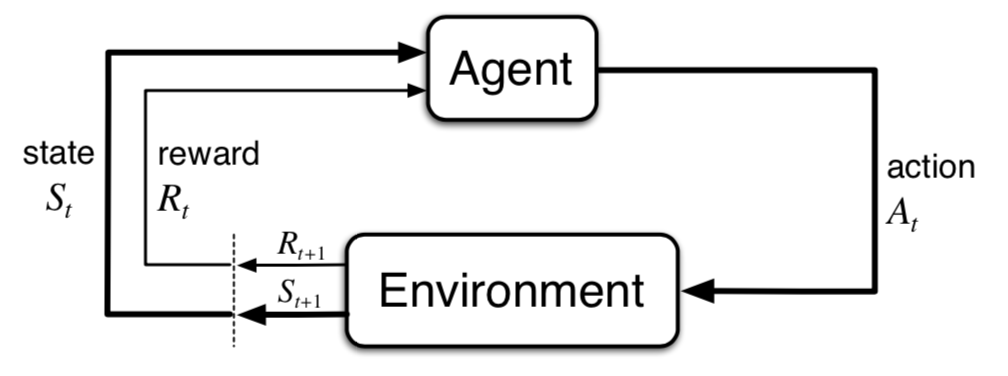
\includegraphics[scale=1]{basicRL.png}
    \caption{Basic overview of the reinforcement learning setting with an agent interacting via actions ($A_t$) with it's environment moving through states ($S_t$). Thus gaining different rewards ($R_t$). Source: \textcite{sutton1998reinforcement} }
    \label{fig:4}
\end{figure}

Reinforcement learning (RL) is about an agent interacting with the environment. By learning an optimal policy, by trial and error. For sequential decision making \parencite{li2017deep}. \autoref{fig:4} above illustrates a simple agent interacting with its environment. A RL agent interacts with its environment over time. At each time step $t$ the agent receives  a \textit{state} $S_t$ in a state space $\mathcal{S}$ and makes an \textit{action} $A_t$ from an action space $\mathcal{A}$ \parencite{li2017deep}. As a consequence of its action, the agent receives \textit{reward} $R_t$ which is a scalar value. The agent's goal is to maximize the total amount of cumulative reward it receives. This is know as the \textit{reward hypothesis} \parencite{sutton1998reinforcement}. The agent's behavior is modelled by the \textit{policy} $\pi(s|a)$. A policy is a mapping from a state to an action, that is the probability of selecting action $A_t=a$ if state $S_t = s$. 
\newline
\newline
This also includes transitioning to the next state $S_{t+1}$ according to the environments dynamics or \textit{model} for a \textit{reward function} $\mathcal{R}(s,a)$ and \textit{state transition probability}
\subsubsection*{Markov Decision Process}
$\mathcal{P}(S_{t+1} |S_t, A_t)$ \parencite{li2017deep}. More formally the RL problem is formulated as an \textit{Markov Decision Process} (MPD) \parencite{sutton1998reinforcement, li2017deep}. A MDP is a tuple $(\mathcal{S, A, P, R}, \gamma)$ \parencite{li2017deep}:
\begin{itemize}
    \item $\mathcal{S}$ is a finite set of states
    \item $\mathcal{A}$ is a finite set of actions
    \item $\mathcal{P}$ is a transition probability matrix, 
    \begin{equation} 
        \label{eq:12a}
        \mathcal{P}^{a}_{ss'} = P[S_{t+1} = s' | S_t =s, A_t = a]
    \end{equation}
    \item $\mathcal{R}$ is a reward function, 
    \begin{equation}
        \label{eq:12b}
        \mathcal{R}^{a}_{s} = E[R_{t+1} | S_t =s, A_t=a]
    \end{equation}
    \item $\gamma \in [0,1]$ is a \textit{discount factor} 
\end{itemize}
In general, we seek to maximize the \textit{expected return}. Where the return, denoted $G_t$ is total discounted reward from time step $t$:

\begin{equation}
    \label{eq:13}
    G_t = R_{t+1} + \gamma R_{t+2} + ... = \sum_{k=0}^{\infty}{\gamma^{k}R_{t+k+1}}
\end{equation}
The discount factor or discount rate in \autoref{eq:13} determines the present value of future rewards, $k$ steps in the future. Note that a $\gamma$ close to 0 leads to \textit{myopic} behavior i.e. the agent only cares about immediate rewards. Whilst if $\gamma$ is close to 1, the agent's is a bit more \textit{far-sighted}. When the agent-environment interaction breaks naturally into sub-sequences which is called \textit{episodes}
\autoref{eq:13} makes sense. 

\subsubsection*{Value Functions}

Almost all RL algorithms involve estimating \textit{value functions} i.e. functions of states or state-action pairs. These estimate how god it is for an agent to be in a certain state \parencite{sutton1998reinforcement, li2017deep}. The value of a state $s$ under a policy $\pi$ denoted $v_{\pi}(s)$. Is the expected return when starting in $s$ and following $\pi$. Below is the \textit{state-value function for policy $\pi$}:

\begin{equation}
    \label{eq:14}
    v_{\pi}(s) = E_{\pi}[G_t | S_t = s] = E_{\pi}\left[\sum_{k=0}^{\infty}{\gamma^{k}R_{t+k+1}} | S_t = s\right], \forall s \in \mathcal{S}.
\end{equation}
Note that the value of the terminal state is always zero \parencite{sutton1998reinforcement}. Similarly  we can define the the \textit{action-value function for policy $\pi$} \parencite{sutton1998reinforcement}. Which is the value of taking action $a$ in state $s$ under policy $\pi$, denoted $q_{\pi}(s,a)$. Is the expected return starting from $s$, taking the action $a$ and therefore following policy $\pi$:

\begin{equation}
    \label{eq:15}
    q_{\pi} = E_{\pi}[G_t | S_t =s, A_t = a] = E_{\pi} \left[\sum_{k=0}^{\infty}{\gamma^{k}R_{t+k+1}} | S_t=s, A_t=a \right]
\end{equation}
Both \autoref{eq:14} and \autoref{eq:15} can be estimated from experiences or by using \textit{Monte Carlo Methods} \parencite{sutton1998reinforcement}.

\subsubsection*{Bellman equations \& Optimality}
Both \autoref{eq:14} and \autoref{eq:15} satisfies recursive relationships. Which is commonly know as \textit{Bellman equations} \parencite{sutton1998reinforcement}:

\begin{equation}
    \label{eq:16}
    v_{\pi} = E[G_t | S_t = s] = E_{\pi}[R_{t+1} + \gamma G_{t+1} | S_t = s]
\end{equation}

\begin{equation}
    \label{eq:17}
    q_{\pi} = E_{\pi}[R_{t+1} + \gamma G_{t+1} | S_t = s,  A_t = a]
\end{equation}
As we can see in \autoref{eq:16} and \autoref{eq:17} the Bellman equations expresses a relationship between the value of the state and its successor states. However solving a RL task means that we want to find a policy that achieves a lot of reward over the long run. We are thus looking for \textit{optimal policies} ($\pi \geq \pi'$). We denote all optimal policies with $\pi_{*}$ whom share the same state-value and action value-value functions \parencite{sutton1998reinforcement}. We thus want to maximize the following:

\begin{equation}
    \label{eq:18}
    v_{*}(s) = \underset{\pi}{\text{max }} v_{\pi}(s)
\end{equation}

\begin{equation}
    \label{eq:19}
    q_{*}(s,a) = \underset{\pi}{\text{max }} q_{\pi}(s,a)
\end{equation}

Using \autoref{eq:18} and \autoref{eq:19} together with the Bellman equation in \autoref{eq:16} and \autoref{eq:17} we get the \textit{Bellman optimality equations}:

\begin{equation}
\label{eq:20}
\begin{aligned}
& & v_{*}(s) =  \underset{a}{\text{max }} 
E_{\pi_{*}}[R_{t+1} + \gamma v_{*}(S_{t+1}) | S_t =s, A_t = a] \\
& & = \underset{a}{\text{max }} 
\sum_{s', r}^{}{p(s', r | s,a)}[r + \gamma v_{*}(s')]
\end{aligned}
\end{equation}

\begin{equation}
\label{eq:21}
\begin{aligned}
& & q_{*}(s,a) = 
E[R_{t+1} + \gamma \underset{a'}{\text{max }}q_{*}(S_{t+1, a'}) | S_t =s, A_t = a] \\
& & =  \sum_{s', r}^{}{p(s', r | s,a)}[r + \gamma \underset{a'}{\text{max }}q_{*}(s',a')]
\end{aligned}
\end{equation}
For a finite MDP \autoref{eq:20} and \autoref{eq:21} has a unique solution independent of the policy \parencite{sutton1998reinforcement}. Nevertheless, in practice there is no closed form solution for these equations. Therefore one must resort to approximate and iterative methods. That uses \textit{dynamic programming} or Monte Carlo methods.

\subsection{Exploration versus Exploitation}
In reinforcement learning we have a trade-off between \textit{exploration} and \textit{exploitation}. Where exploration refers to taking actions, that come from the current best version of the learned policy. Exploration instead is concerned with taking more actions to obtain more training data \parencite{goodfellow2016deep}. Where the dilemma is that neither exploration nor exploitation can be pursued exclusively without failing at the task \parencite{sutton1998reinforcement}.

\subsection{Algorithms \& Learning in RL}
One can characterize RL problems into two main classes: \textit{prediction} and \textit{control} where each is followed by different approaches as \textit{value iteration, policy iteration} and \textit{policy search} \parencite{szepesvari2009algorithms}. These different approaches uses different algorithms 

\subsection{Competitive Self-Play}

%mention where it has been succesfully used and show the need of the application that we want to use here for the thesis
\subsection{RL in Market Microstructure}

\subsection{Issues with deep RL}


%necessary?
%\section{Tree Search}

%\subsection{MinMax}

%\subsection{Monte Carlo Tree Search (MCTS)}

%own chapter?
\section{Related Work}


\chapter{Methods}

\chapter{Experiments}

\chapter{Results}

\chapter{Discussion \& Conclusions}

\printbibliography[heading=bibintoc] % Print the bibliography (and make it appear in the table of contents)

\appendix

\chapter{Unnecessary Appended Material}

\end{document}
